\documentclass[lang=cn,11pt,a4paper,cite=authornum]{paper}

\title{操作系统 实验:多线程编程 \\ 实验报告}
\author{毛子恒 \\ 2019211397}
\institute{北京邮电大学\ 计算机学院}

\date{\zhtoday}

% 本文档命令
\nocite{*}

\begin{document}

\maketitle

\section{概览}

\subsection{实验内容}

给定两个矩阵$\mathbf{A}_{N\times K}$和$\mathbf{B}_{K\times M}$,它们的矩阵积为$\mathbf{C}_{N\times M}$定义为:

$$
C_{i,j}=\sum_{n=1}^{K}A_{i,n}\times B_{n,j}
$$

给出矩阵$\mathbf A$和矩阵$\mathbf B$,计算$\mathbf C$。其中计算每个$C_{i,j}$是一个独立的工作线程。

\subsection{实验环境}

\begin{itemize}
    \item openEuler 20.03 64bit with ARM
    \item gcc version 7.3.0
    \item vim 8.1
\end{itemize}

\section{实验设计}

\subsection{相关API}

\begin{itemize}
    \item \mintinline{C}{int pthread_attr_init(pthread_attr_t *attr);}:用默认的属性参数初始化指向\mintinline{text}{attr}的线程属性对象,如果成功,返回0。
    \item \mintinline{C}{int pthread_create(pthread_t *restrict thread, const pthread_attr_t *restrict attr, void *(*start_routine)(void *), void *restrict arg);}:在当前进程创建一个新线程,新线程通过唤起\mintinline{text}{start_routine}开始执行,\mintinline{text}{arg}参数被传递到\mintinline{text}{start_routine}的参数,\mintinline{text}{attr}指向的结构体的内容用来决定新线程创建时的一些参数,如果为\mintinline{text}{NULL},则采用默认参数。在该函数返回之前,新线程的ID将被存储到\mintinline{text}{thread}中。当成功时,该函数返回0。
    \item \mintinline{C}{noreturn void pthread_exit(void *retval);}:该函数终止调用它的线程,并且通过\mintinline{text}{retval}给当前进程中调用\mintinline{C}{pthread_join()}的另一个线程返回一个值。
    \item \mintinline{C}{int pthread_join(pthread_t thread, void **retval);}:该函数等待\mintinline{text}{thread}指定的线程终止,如果这个线程已经终止,则该函数立即返回。如果\mintinline{text}{retval}不是\mintinline{text}{NULL},则该函数复制目标线程给\mintinline{text}{pthread_exit()}的参数到\mintinline{text}{retval}所指向的地址。如果成功,该函数返回0。
    \item \mintinline{C}{int pthread_attr_destroy(pthread_attr_t *attr);}:销毁\mintinline{text}{pthread_attr_init()}创建的线程属性对象。销毁一个正在被某个线程使用的参数对象不会产生影响。如果成功,该函数返回0。
\end{itemize}

\subsection{设计概述}

\begin{figure}[htbp]

    \centering
    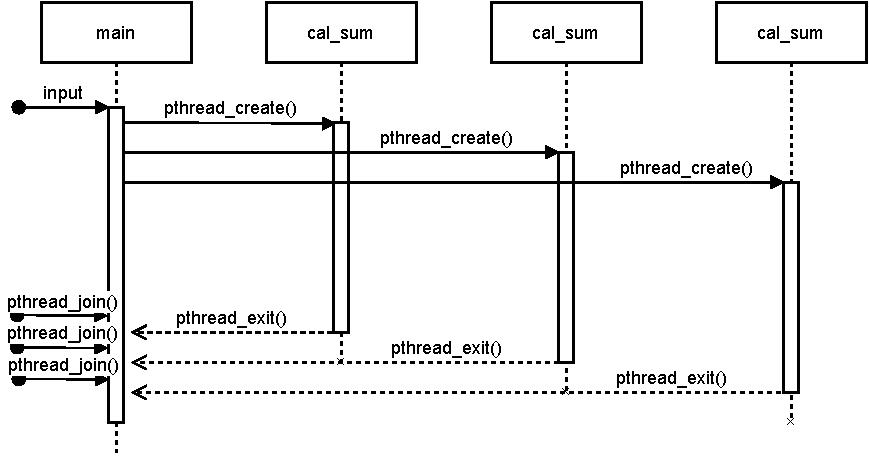
\includegraphics[width=0.8\linewidth]{./images/UML1.pdf}
    \caption{时序图\label{fig:UML1}}

\end{figure}

如\figref{fig:UML1}所示,主线程首先通过标准输入读取$n,k,m$和$\mathbf A,\mathbf B$两个矩阵,在此期间分配三个矩阵的内存空间。之后,程序分配数组\mintinline{text}{tid}用于存储线程ID,并且初始化线程属性对象。

程序通过循环遍历$\mathbf C$的每一个位置,在循环中创建一个\mintinline{C}{struct v}类型的对象,之后通过\mintinline{C}{pthread_create()}创建线程,线程调用\mintinline{C}{cal_sum()}函数,将\mintinline{C}{struct v}类型的对象作为参数传递给该函数。\mintinline{C}{struct v}结构体的定义如下:

\begin{code}
\begin{minted}{C}
struct v
{
    int i, j;
};
\end{minted}
\end{code}

工作线程执行\mintinline{C}{cal_sum()}函数,该函数可以通过提取参数来获得需要求的数字是$C_{i,j}$,之后该函数遍历$\mathbf A$的第$i$行和$\mathbf B$的第$j$列,求出$C_{i,j}$,将结果存储到全局变量\mintinline{C}{c[i][j]}中。最后,工作线程终止。

创建完各个工作线程之后,主线程调用\mintinline{C}{pthread_join()}等待各个工作线程终止。之后向标准输出中打印结果,销毁线程属性对象,并且释放内存。

\section{运行结果及分析}

\subsection{输入}

\begin{code}
\begin{minted}{text}
3 2 3
1 4 2 5 3 6
8 7 6 5 4 3
\end{minted}
\end{code}

\subsection{输出}

\begin{code}
\begin{minted}{text}
28 23 18 
41 34 27 
54 45 36
\end{minted}
\end{code}

\subsection{分析}

\begin{figure}[htbp]

    \centering
    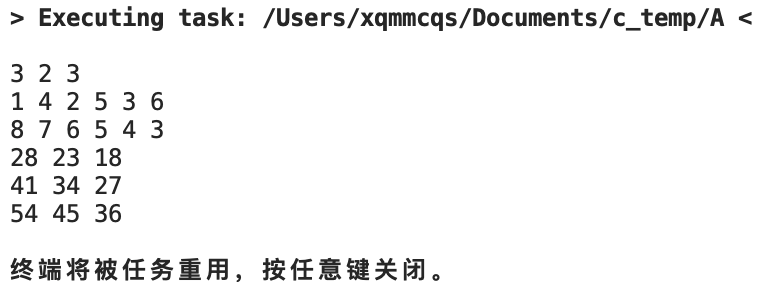
\includegraphics[width=0.6\linewidth]{./images/running.png}
    \caption{运行截图}

\end{figure}

主线程成功创建了各个工作线程,工作线程计算出答案后,主线程正确输出。

\section{实验总结}

本次实验中我利用POSIX API编写了三个与线程控制的程序,使我对相关知识点的掌握更加牢固。

我通过查阅\href{https://man7.org/linux/man-pages/index.html}{Linux man page}获取相关API的信息,并且参考教材的内容编写程序。在阅读man page和相关文档的过程中我对用户线程的线程控制和线程的内存共享有了更多的认识。

本次实验使我的C编程能力和英文文献阅读能力得到提高,我从中收获颇丰。

\end{document}